\documentclass{standalone}
\usepackage{tikz}
\begin{document}
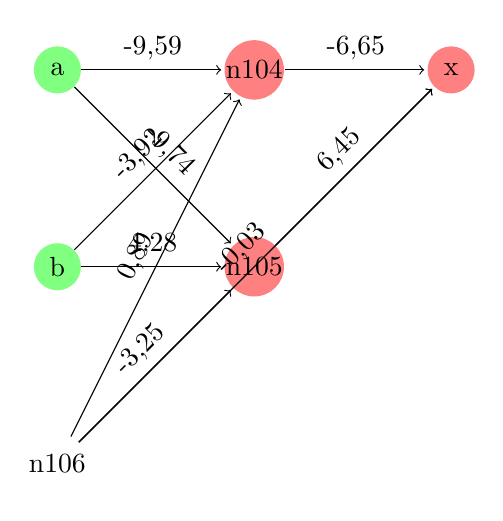
\begin{tikzpicture}[shorten >=1pt,->,draw=black!,node distance=2.5cm]
\tikzstyle{neuron}=[circle,fill=black!25,minimum size=17pt,inner sep=0pt]
\tikzstyle{constant}=[neuron, fill=white!50];
\tikzstyle{identity}=[neuron, fill=green!50];
\tikzstyle{sigmoid}=[neuron, fill=red!50];
\node [identity] (a) {a};
\node [identity,below of=a] (b) {b};
\node [constant,below of=b] (n106) {n106};
\node [sigmoid,right of=a] (n104) {n104};
\node [sigmoid,below of=n104] (n105) {n105};
\node [sigmoid,right of=n104] (x) {x};
\path[every node/.style={sloped,anchor=south,auto=false}]
(a) edge node {-9,59} (n104)
(a) edge node {-9,74} (n105)
(b) edge node {4,28} (n105)
(b) edge node {-3,92} (n104)
(n106) edge node {-0,03} (x)
(n106) edge node {0,89} (n104)
(n106) edge node {-3,25} (n105)
(n104) edge node {-6,65} (x)
(n105) edge node {6,45} (x)
;\end{tikzpicture}
\end{document}